\chapter{DETAILED DESIGN}

\section{Architectural Design}
	\begin{figure}[h!]
		\centering
		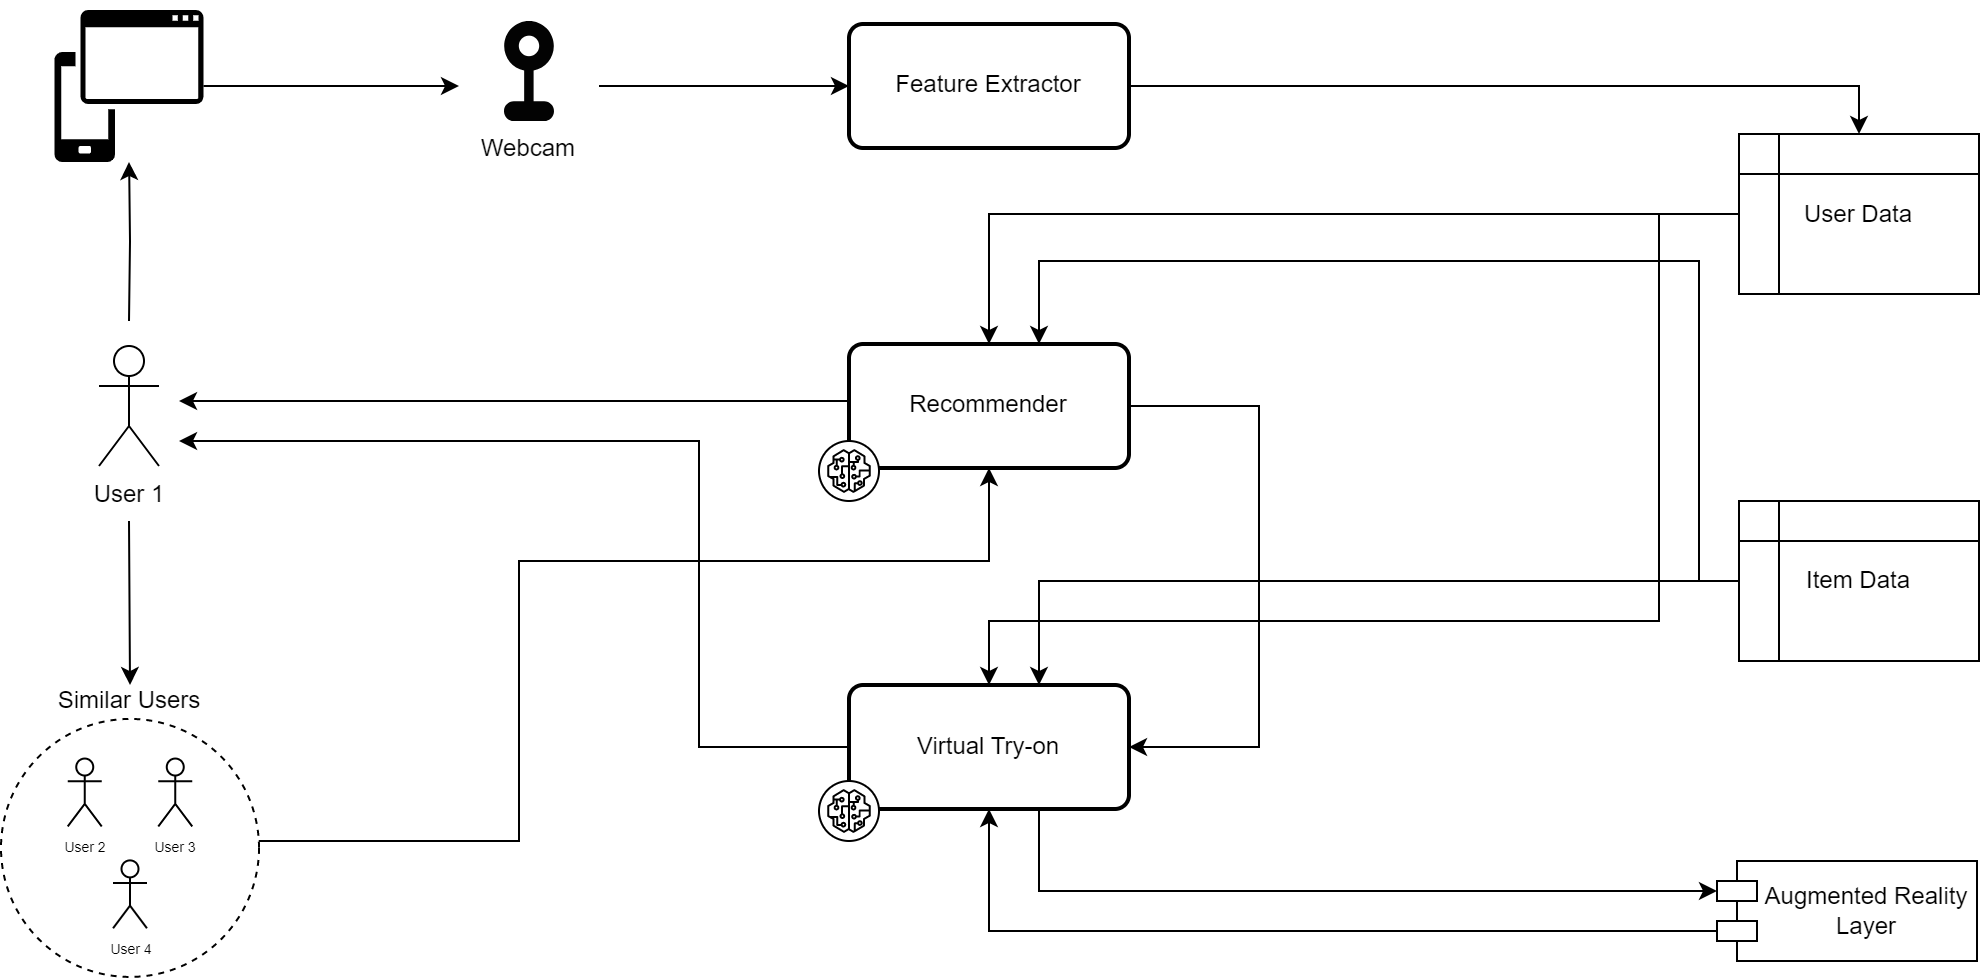
\includegraphics[width=0.75\textwidth]{components/images/sys-arch.png}
		\caption{System Architecture}
		\label{fig:sys-arch}
	\end{figure}

\section{UML Diagrams}
	\subsection{Use-case Diagram}
		\begin{figure}[h!]
			\centering
			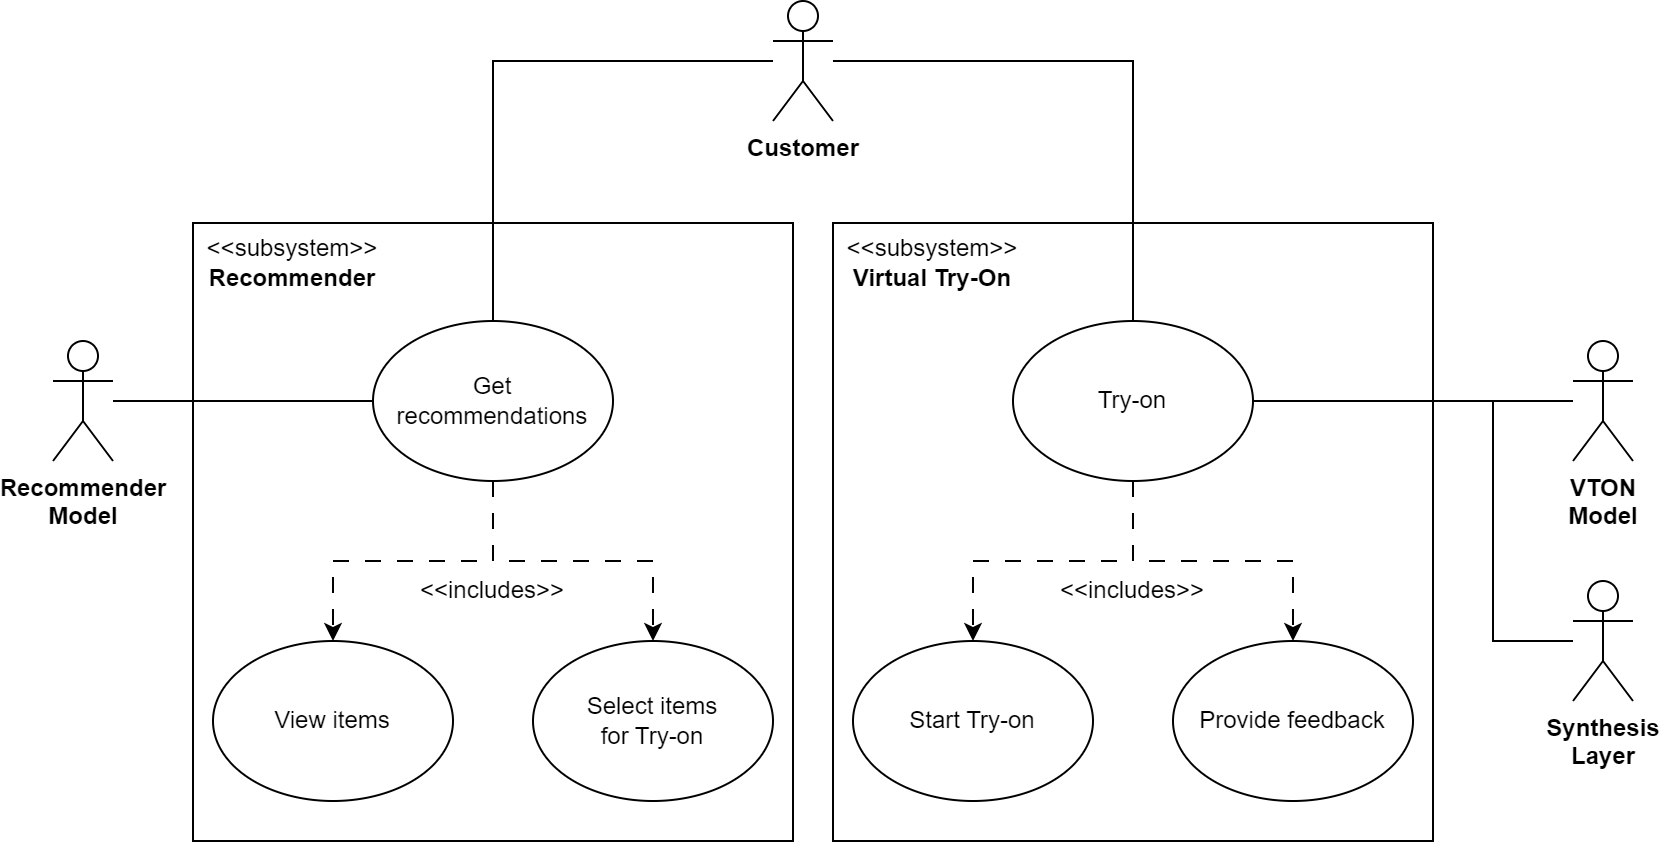
\includegraphics[width=0.75\textwidth]{components/images/use-case.png}
			\caption{Use-case Diagram}
			\label{fig:use-case-rep}
		\end{figure}

	\pagebreak

	\subsection{Sequence Diagram}
		\begin{figure}[h!]
			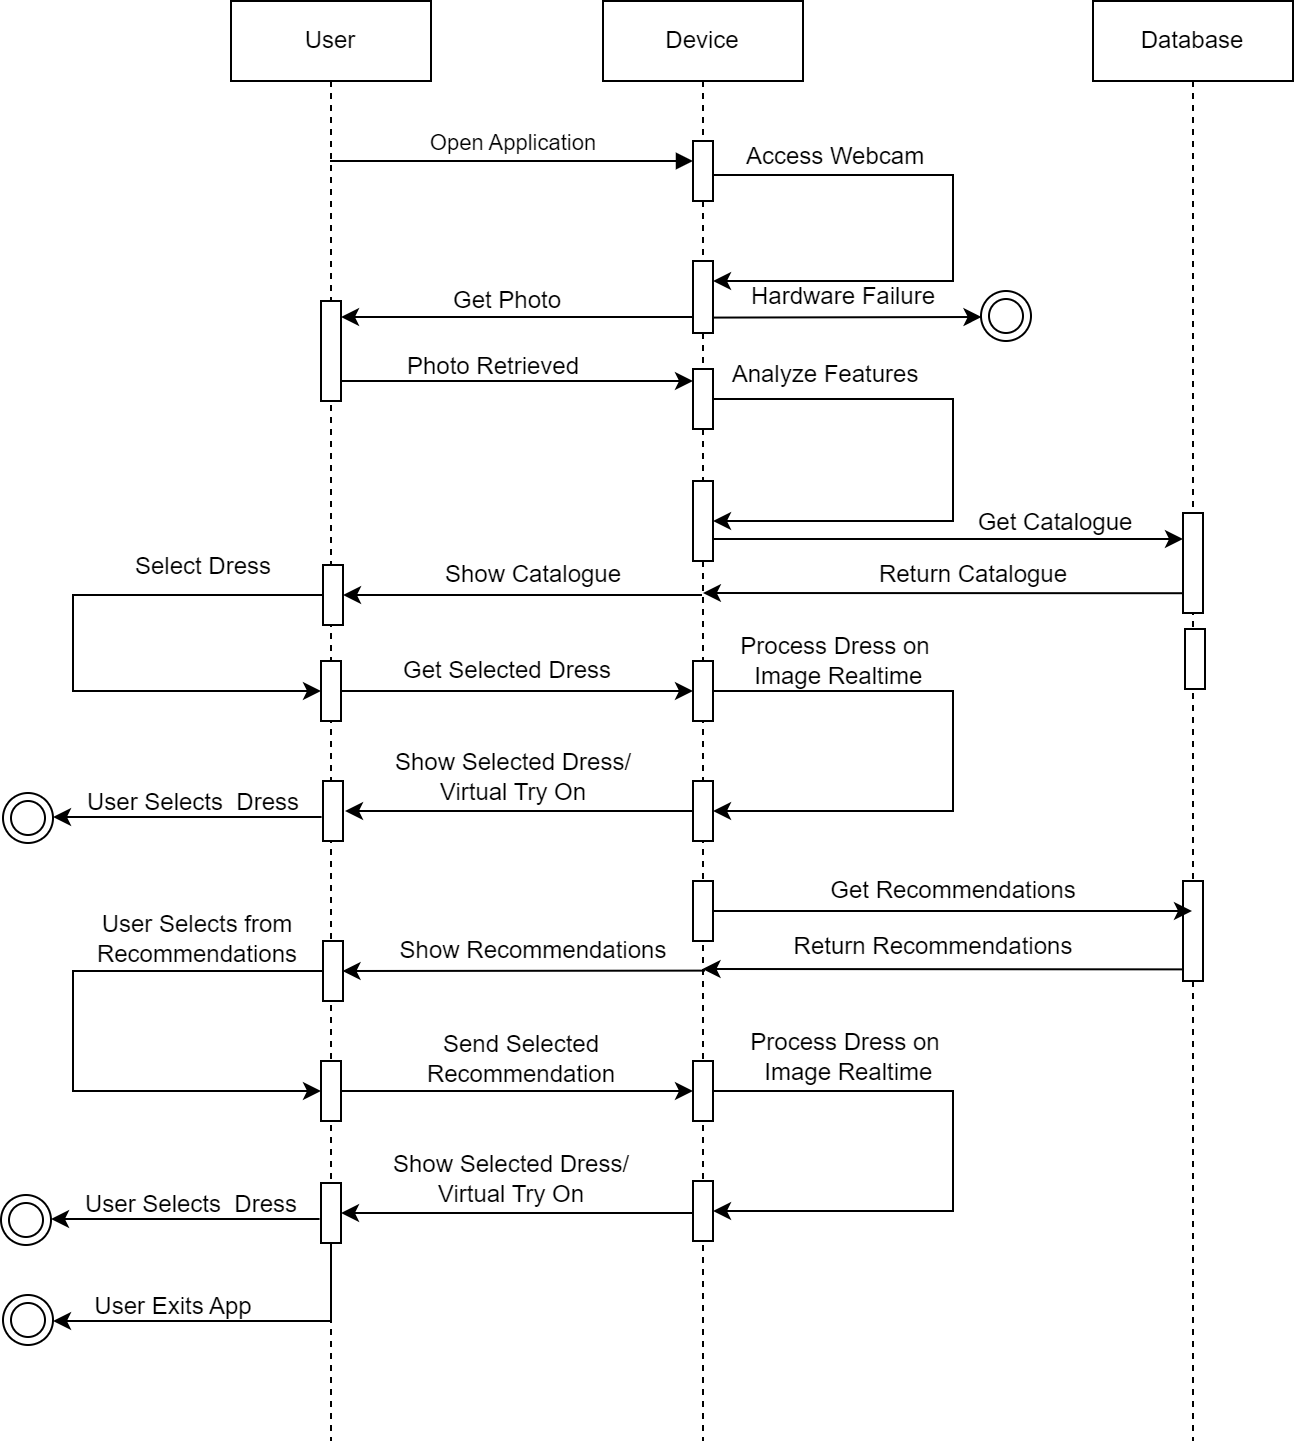
\includegraphics[width=\textwidth]{components/images/sequence.png}
			\caption{Sequence Diagram}
			\label{fig:sequence}
		\end{figure}

	\pagebreak

	\subsection{Activity Diagram}
		\begin{figure}[h!]
			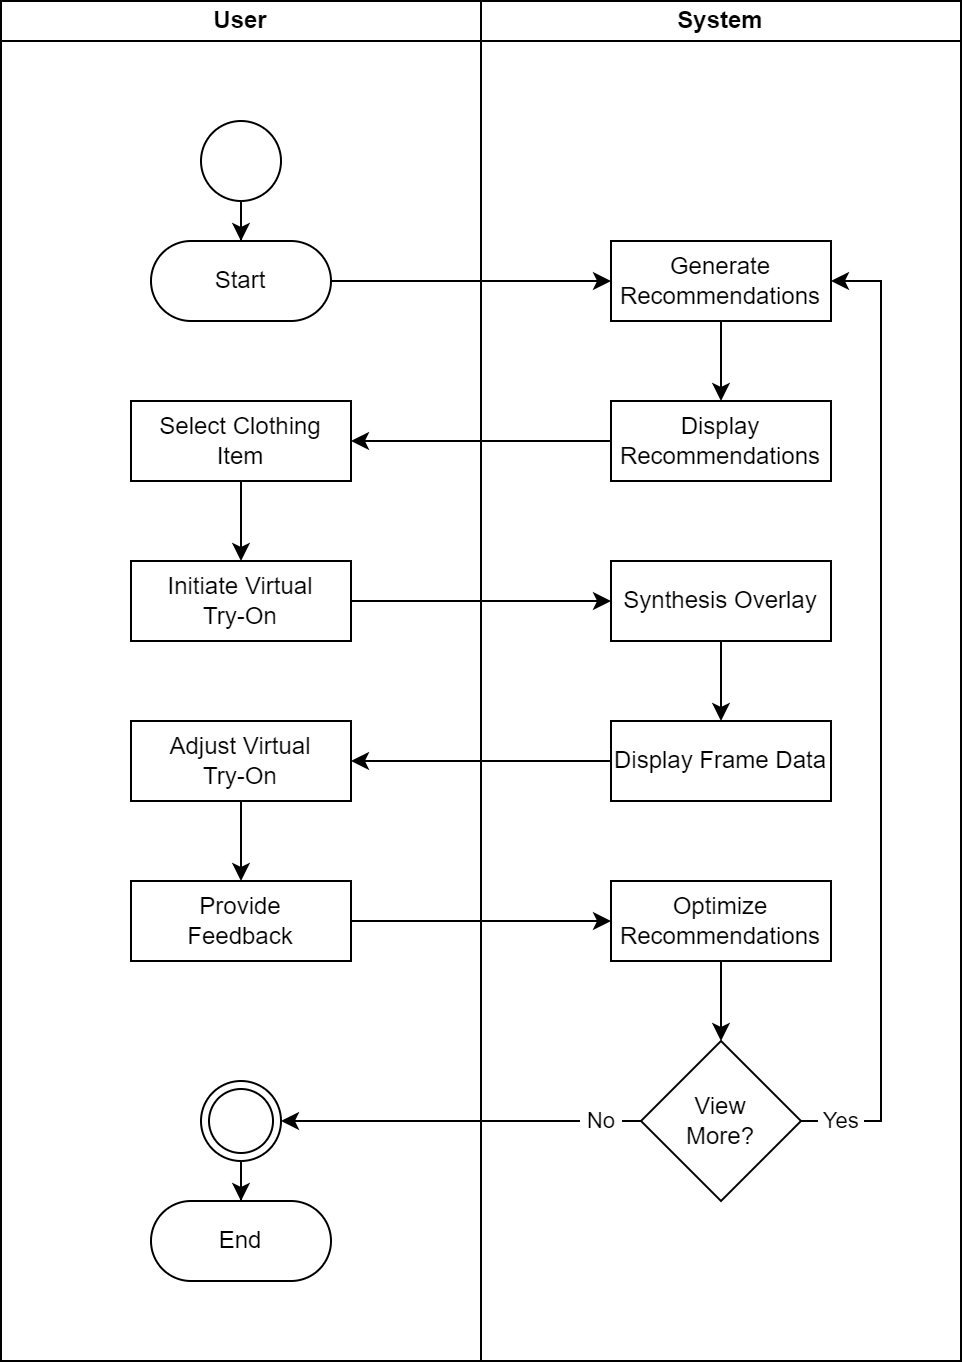
\includegraphics[width=\textwidth]{components/images/activity.png}
			\caption{Activity Diagram}
			\label{fig:activity}
		\end{figure}

	\pagebreak

	\subsection{State Diagram}
		\begin{figure}[h!]
			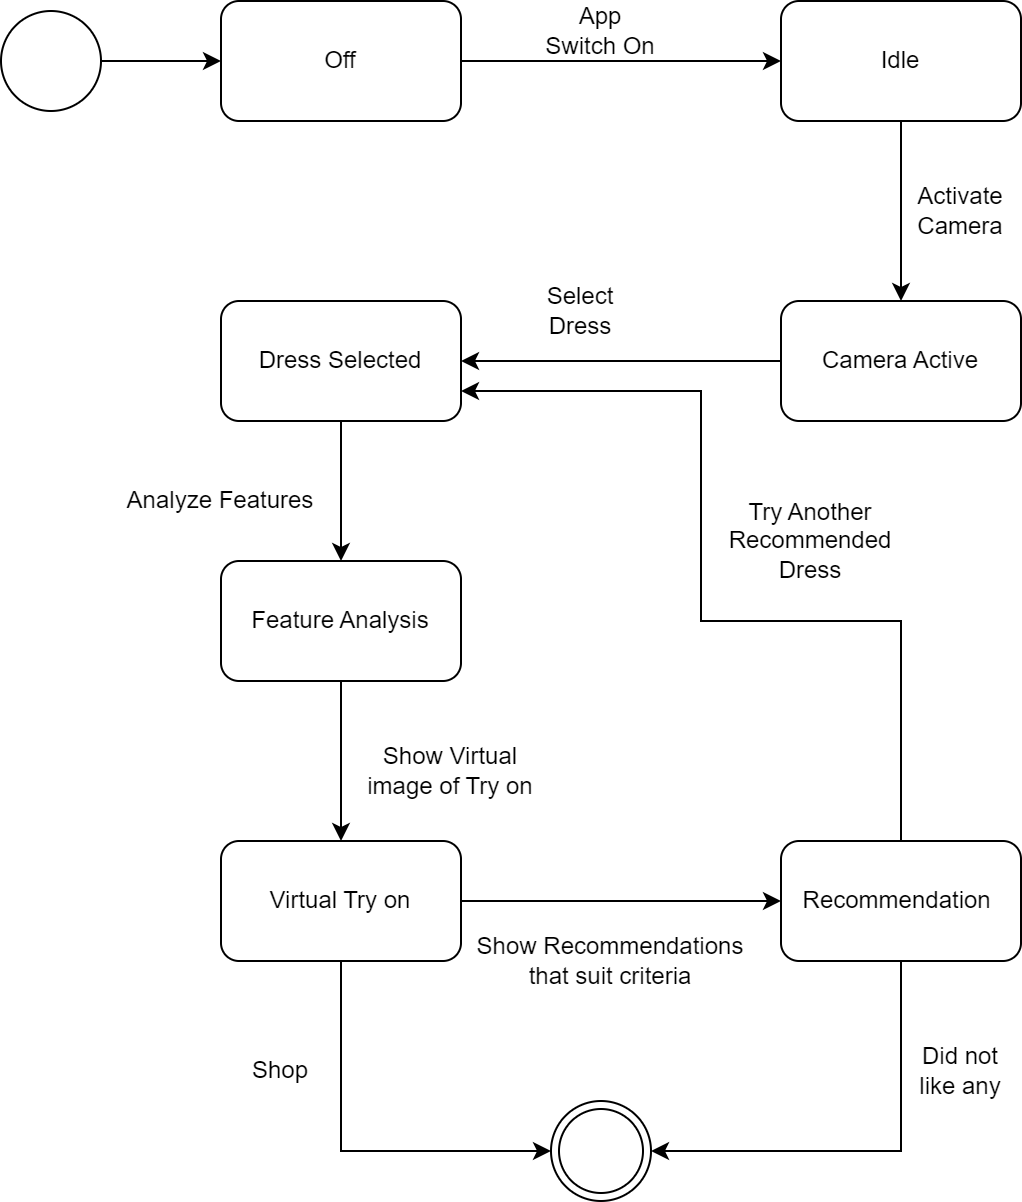
\includegraphics[width=\textwidth]{components/images/state.png}
			\caption{State Diagram}
			\label{fig:state}
		\end{figure}

	\pagebreak

	\subsection{Component Diagram}
		\begin{figure}[h!]
			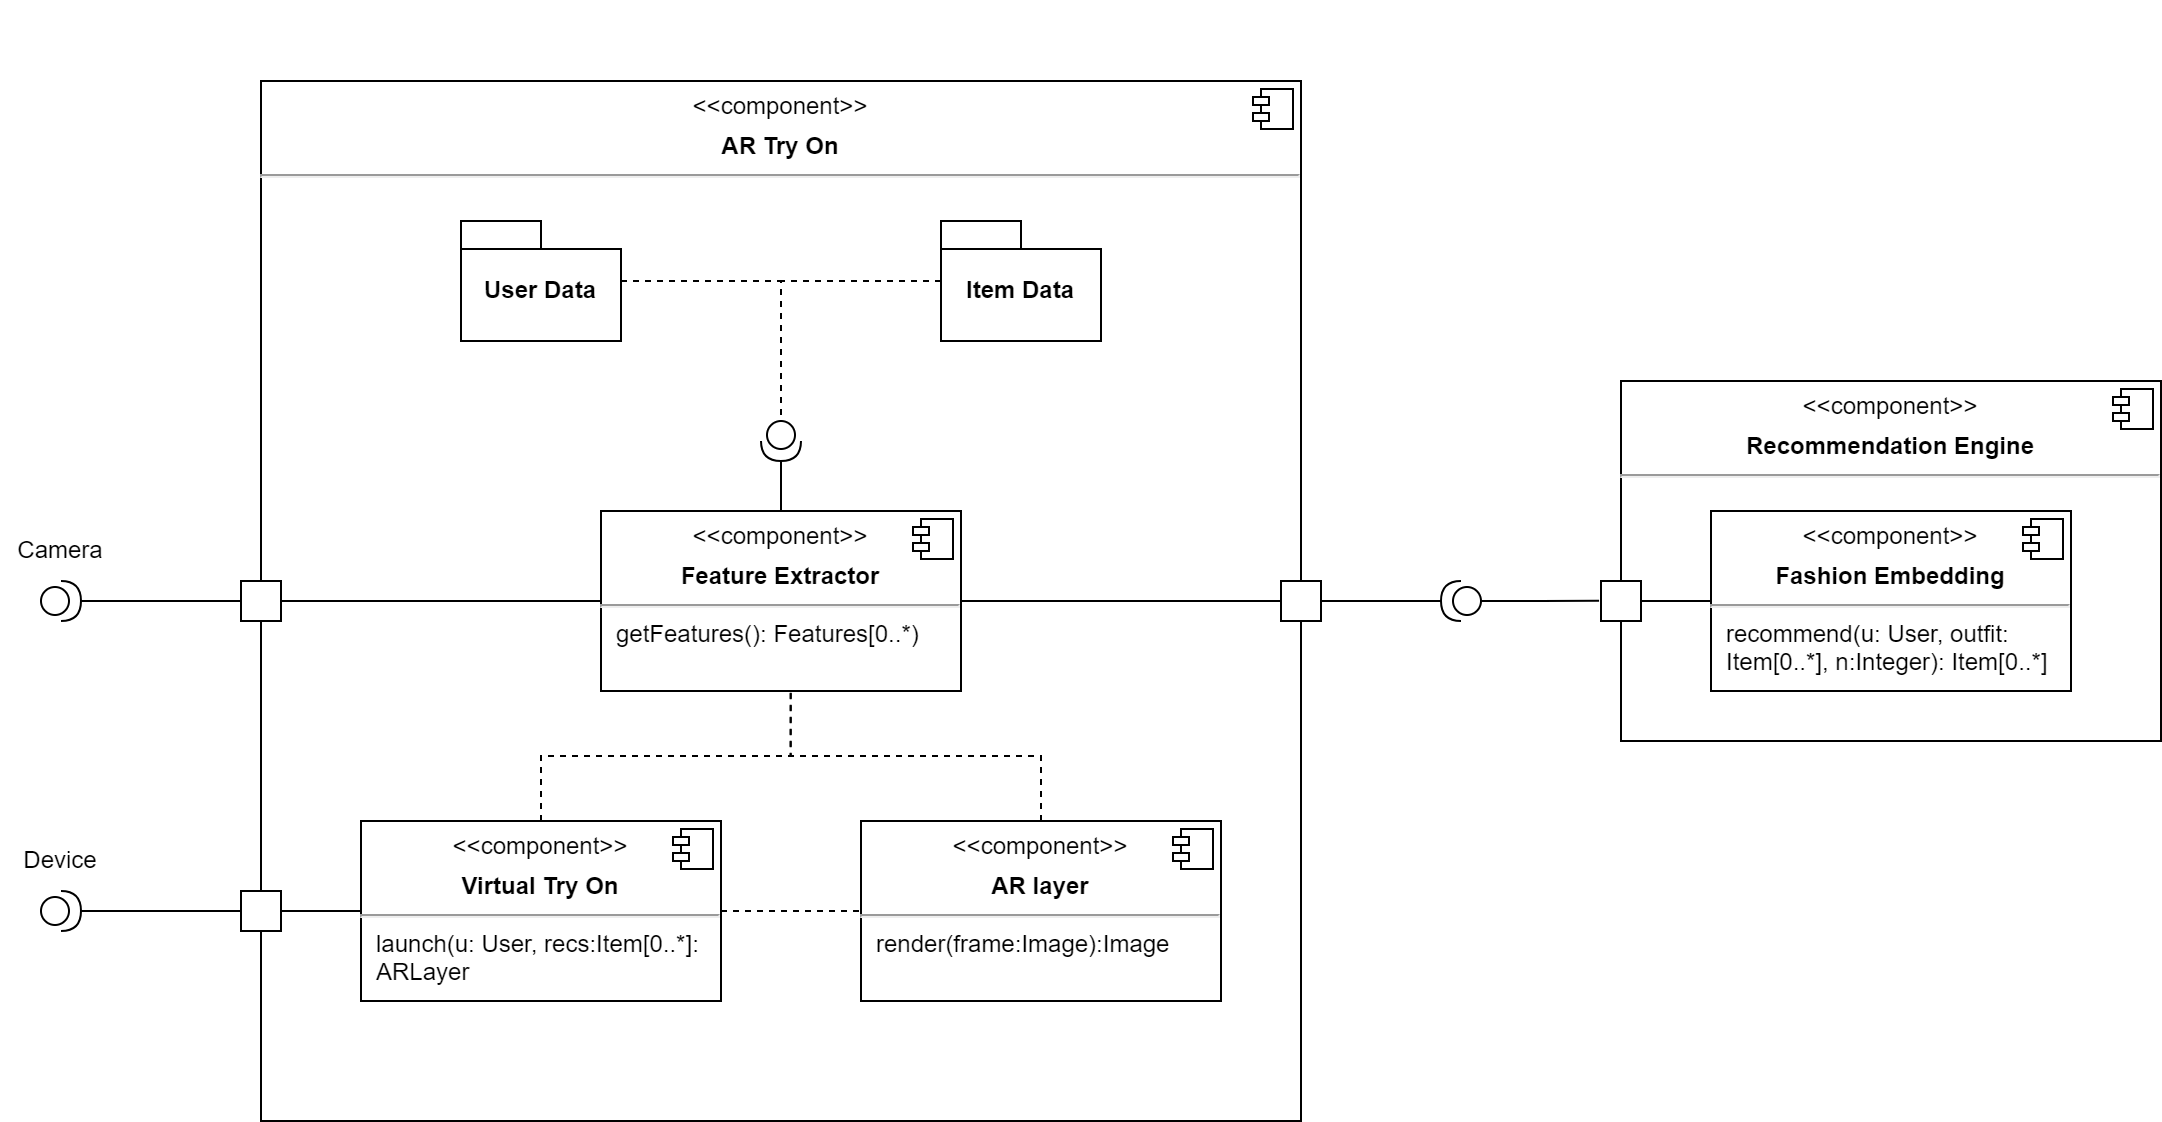
\includegraphics[width=\textwidth]{components/images/component.png}
			\caption{Component Diagram}
			\label{fig:component}
		\end{figure}

	\subsection{Class Diagram}
		\begin{figure}[h!]
			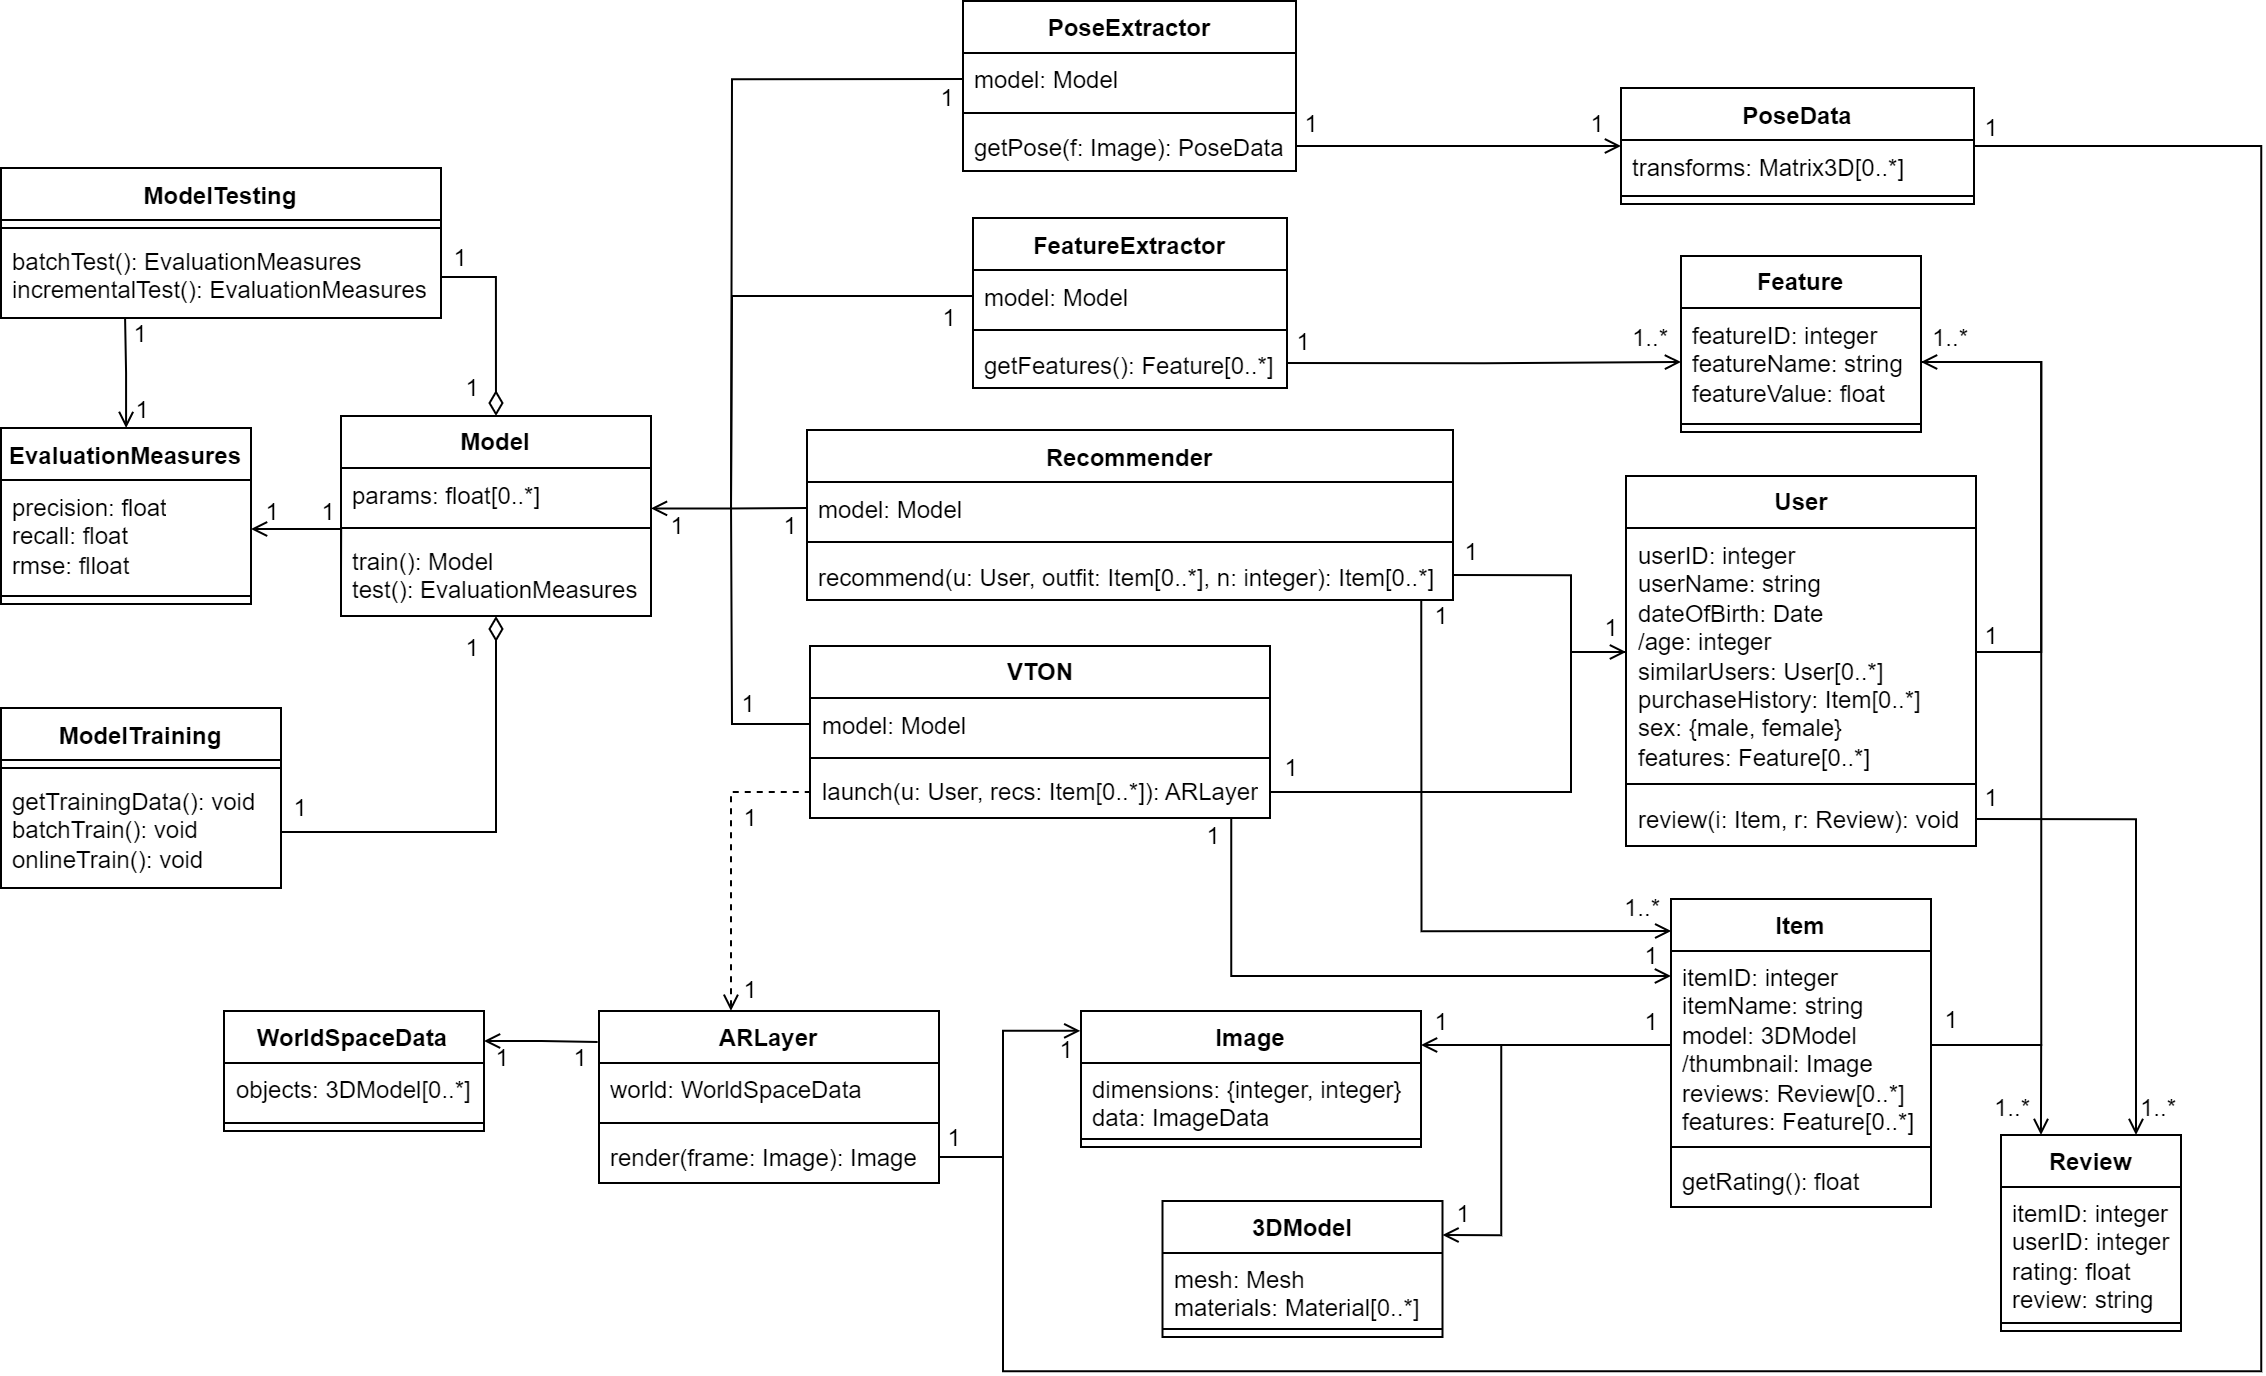
\includegraphics[width=\textwidth]{components/images/class.png}
			\caption{Class Diagram}
			\label{fig:class}
		\end{figure}

	\pagebreak

	\subsection{Object Diagram}
		\begin{figure}[h!]
			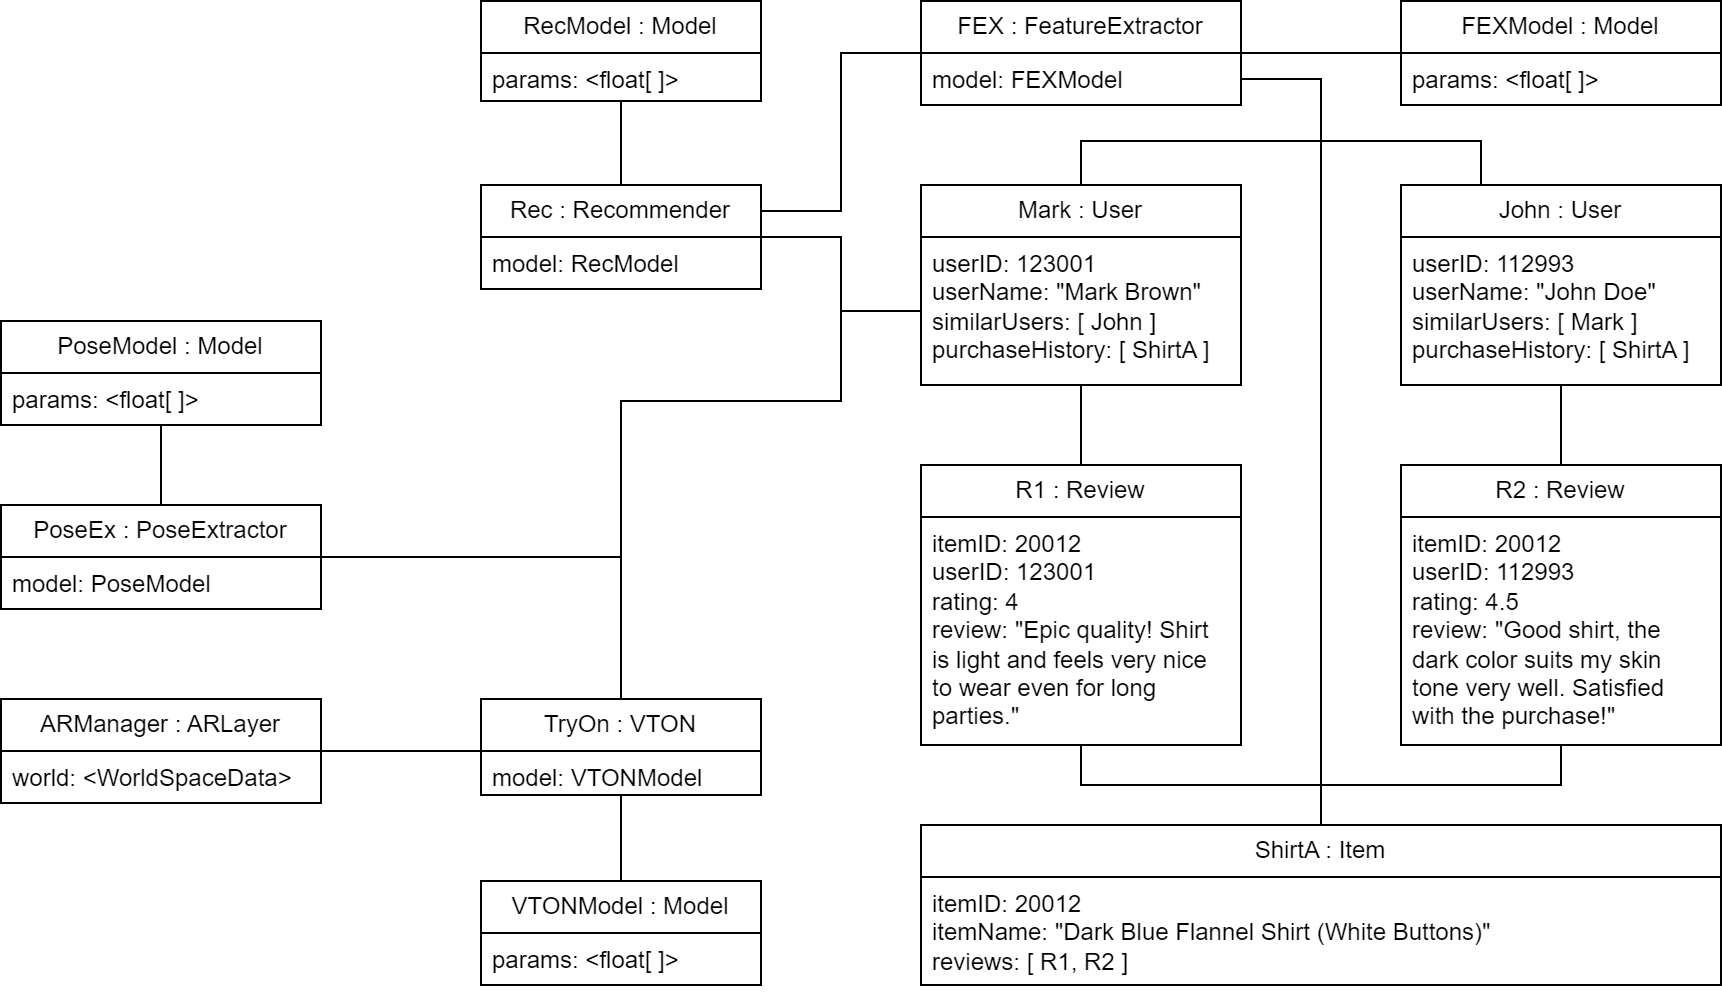
\includegraphics[width=\textwidth]{components/images/object.png}
			\caption{Object Diagram}
			\label{fig:object}
		\end{figure}

	\subsection{Deployment Diagram}
		\begin{figure}[h!]
			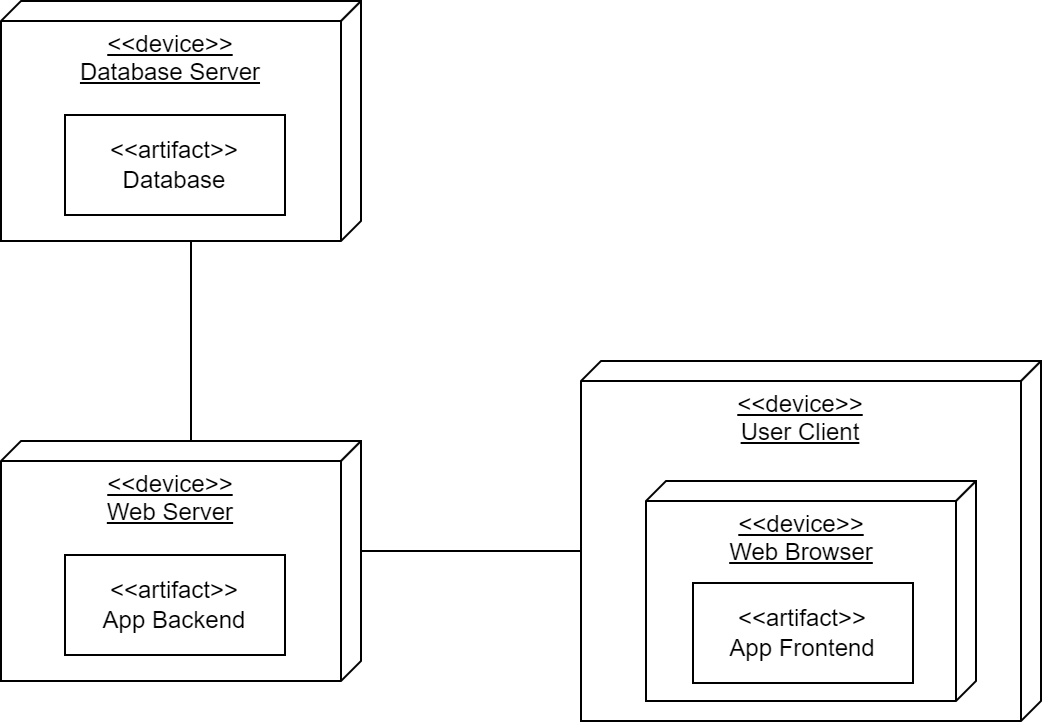
\includegraphics[width=\textwidth]{components/images/deployment.png}
			\caption{Deployment Diagram}
			\label{fig:deployment}
		\end{figure}